% !TeX spellcheck = <none>
\documentclass[10pt,a4paper]{article}
\usepackage[utf8]{inputenc}
\usepackage{amsmath}
\usepackage{amsfonts}
\usepackage{amssymb}
\usepackage{graphicx}
\usepackage{bm}
%%% formatting the code
\usepackage{listings}



\usepackage{color}
\lstset{%
	escapeinside={(*}{*)},%
}

\newcommand{\amidstversion}{\input{../../version.txt}}

\lstset{
	frameround=fttt,
%	language=java,
	numbers=left,
	breaklines=true,
	mathescape, 
	columns=fullflexible, 
	basicstyle=\fontfamily{lmvtt}\selectfont,
	keywordstyle=\color{blue}\fontfamily{lmvtt}\selectfont, 
	numberstyle=\color{black}
}
\lstMakeShortInline[columns=fixed]|



\newcommand{\includejavasource}[1]{\lstinputlisting[language=java]{#1}}
\newcommand{\inlinejava}[1]{\lstinline[columns=fixed,language=java]{#1}}

\newcommand{\lang}[1]{}



\usepackage{hyperref}



\begin{document}

\section{Probabilistic Graphical Models on Multi-Core CPUs Using Java 8}\label{sec:blog:multicore}
%\subsection{Introduction}\label{sec:lvmodels:intro}

Herein we discuss software design issues related to the development of parallel computational intelligence algorithms on multi-core CPUs, using the new Java 8 functional programming features. In particular, we focus on probabilistic graphical models (PGMs) and present the parallelisation of a collection of algorithms that deal with inference and learning of PGMs from data. For a more details, you can check the following article:

\begin{quotation}
Masegosa, A. R., Martinez, A. M., \& Borchani, H. (2016). Probabilistic Graphical Models on Multi-Core CPUs using Java 8. IEEE Computational Intelligence Magazine, 11(2), 41-54.
\end{quotation}

In the following sections, we will illustrate the use of Java 8 and PGMs with a set of code-examples. For that, you will have to download the AMIDST Toolbox from \href{http://www.amidsttoolbox.com/documentation/0-5-2/first-steps-052/getting-started-052/}{here}. 

\subsection{Parallel programming in Java 8}\label{sec:blog:multicore:java8}

The latest Java release (JDK 8.0, March 2014) is an attempt to bring a new API to code transparent and seamless parallel applications to the general public (that is, non-specialized programmers in parallel and concurrent methods). To handle this, Java 8 introduces a completely new approach to parallelism based on a functional programming style through the use of map-reduce operations. \newline

The \textit{map} operation applies a stateless user-defined transformer function (mapper) to each element of the collection, whereas the \textit{reduce} operation applies another stateless user-defined function (reducer) that combines the outputs of the mapper to produce a single output result. Both the mapper and the reducer can be concisely described using \textit{lambda} expressions in Java 8.\newline


In the code below, an example of the map-reduce operations is given. In particular, this code counts the number of occurences of each word in a set of documents (i.e. list of strings).

% word-count

\includejavasource{./code/wordCount.java}




In previous code, an object of class \textit{Stream} is created using \textit{Stream.of}. Each element of such stream, which is processed in parallel, is a document (i.e., a string) . Then, from each document in the flow, a stream of words is generated (map operation). The elements are finally collected (reduced) to an object of class \textit{Map<String, Integer>}.\newline

Java 8 allows the definition of inline functions called \textit{lambda expressions}. These can be used to each element in a collection. In the following example, a parallel stream is created from a list of integers. Then, we filter the stream by selecting even numbers. For that, the lambda expression \textit{$i ->i \% 2 == 0$} is applied to each number.\newline 


% number of odd-even
\includejavasource{./code/NumberEvenOdd.java}

\subsection{Data structures for PGMs using Java 8}\label{sec:blog:multicore:pgms}

Based on previous ideas from Java 8, we might consider implement efficient operations over the data structures in a PGM.  In the AMIDST toolbox, a DAG  (i.e., a Directed Acyclic Graph) is represented as a list of \textit{ParentSet} objects, one for each variable defining our PGM model. Two concrete examples are shown below, where we count the number of links in a DAG. We also collect all the children of a given variable. 


% OperationsOverDAG
\includejavasource{./code/OperationsOverDAG.java}

\subsection{Parallelization of learning algorithms}\label{sec:blog:multicore:learning}
Streams in Java 8 allow us to parallelise tasks without having to explicitly deal with threads and their synchronisation. As a consequence, we are able to implement parallel versions of the learning algorithms.\newline  




As an example, we will considet the learning algorithm \href{http://docslide.us/documents/daphne-koller-parameter-estimation-maximum-likelihood-estimation-probabilistic.html}{Maximum Likelihood Estimation (MLE)}. Given a particular data set of i.i.d. samples

\begin{figure}[h!]
	\centering
	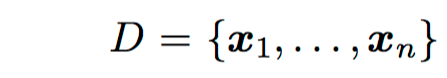
\includegraphics[width=4.5cm]{img/samples.png}
\end{figure}

\noindent and an underlying statistical model, which in our case is a BN whose probability distributions belong to the exponential family, the MLE method gives a unified approach for calculating the parameters of the model that maximize the logarithm of the likelihood function (log-likelihood function) as follows 

\begin{figure}[h!]
	\centering
	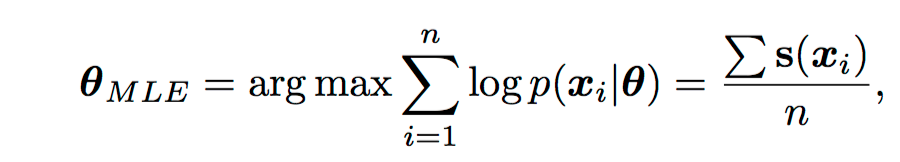
\includegraphics[width=10cm]{img/mle.png}
\end{figure}

\noindent where \textbf{s(xi)} is a deterministic function that returns, for each data sample, a vector of sufficient statistics. For illustrating the implementation of this algorithm, we will learn the parameters of naive Bayes from a random generated dataset with 4 discrete attributes:

\begin{lstlisting}
	int batchSize = 100;
	int seed = 1234;
	int nSamples = 500;
	int nDiscreteAtts = 4;
	int nContAtts = 0;
	
	//Load a data stream
	DataStream<DataInstance> data = DataSetGenerator.generate(seed, nSamples, nDiscreteAtts, nContAtts);
	
	//Generate a DAG with the naive bayes structure
	DAG dag = DAGGenerator.getNaiveBayesStructure(data.getAttributes(), "DiscreteVar0");
	System.out.println(dag);
	

\end{lstlisting}

For computing the sum of all the sufficient statistics (i.e., the numerator in previous equation) we invoke the following method.

\begin{lstlisting}
//Computes the vector of sufficient statistics
CompoundVector sumSS = computeSumSS(data, dag);
\end{lstlisting}

The implementation of the method \textit{computeSumSS} is the following.

\begin{lstlisting}
	public static CompoundVector computeSumSS(DataStream<DataInstance> data, DAG dag) {
		Stream<DataOnMemory<DataInstance>> stream = data.parallelStreamOfBatches(100);
		EF_BayesianNetwork efBayesianNetwork = new EF_BayesianNetwork(dag);
		
		Vector sumSS = stream
			.map(batch -> batch.stream()
				.map(efBayesianNetwork::getSufficientStatistics)
				.reduce(SufficientStatistics::sumVectorNonStateless)
				.get())
			.reduce(SufficientStatistics::sumVectorNonStateless).get();

		return  (CompoundVector)sumSS;
	
	}
\end{lstlisting}


Note that the sum of the vectors of sufficient statistics is computed independent for each batch of data. This is made invoking the method \textit{parallelStreamOfBatches} that returns a parallel stream, i.e., an object of class \textit{Stream<DataOnMemory<DataInstance>>}. Afterwards, the method \textit{map(efBayesianNetwork::getSufficientStatistics)} to each instance in the batch the sufficient statistics vector. The two consecutive calls to \textit{reduce(SufficientStatistics::sumVectorNonStateless).get()} sums the vectors from each instance first, and for each batch later.\newline


If we aim to print the values of the sufficient statistics vector as follows. Note that for computing the estimated probabilities, the vectors must be normalized (i.e., divided by the number of instances).

\begin{lstlisting}

		System.out.println("\nsufficient statistics vectors");
		IntStream.range(0,sumSS.getNumberOfBaseVectors())
			.forEach(
				i -> System.out.println(
					dag.getVariables().getVariableById(i).getName()
					+": "+sumSS.getVectorByPosition(i).output()
			)
		);
		
		
		//Divide by the number of instances
		sumSS.divideBy(data.stream().count());
		
		System.out.println("\nEstimated probabilities:");
		
		//print the estimated probabilities
		IntStream.range(0,sumSS.getNumberOfBaseVectors())
			.forEach(
				i -> System.out.println(
					dag.getVariables().getVariableById(i).getName()
					+": "+sumSS.getVectorByPosition(i).output()
			)
		);

\end{lstlisting}


\end{document}